\section{ROS} \label{sec:ros}

\begin{figure}[h]
	\centering
	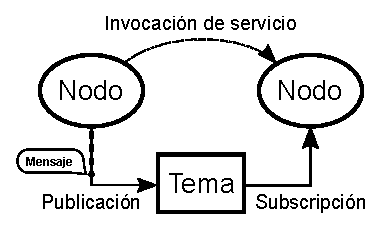
\includegraphics[width=0.5\linewidth]{img/ROS_concepts}
	\caption{Diagrama de comunicación de ROS}
	\label{fig:rosconcepts}
\end{figure}

El \textbf{Robot Operating System (ROS)} es un conjunto de bibliotecas y herramientas de software de código abierto que facilitan el desarrollo de aplicaciones robóticas. Aunque su nombre sugiere que es un sistema operativo, en realidad, ROS actúa como un \textit{middleware} que proporciona servicios similares a los de un sistema operativo, tales como abstracción de hardware, control de dispositivos de bajo nivel, implementación de funcionalidades comunes, paso de mensajes entre procesos y gestión de paquetes. 

\subsubsection{Características principales de ROS}

\begin{itemize}
	\item \textbf{Abstracción de hardware}: Permite a los desarrolladores interactuar con diferentes componentes de hardware sin preocuparse por las especificaciones particulares de cada dispositivo.
	\item \textbf{Sistema de mensajes}: Facilita la comunicación entre procesos mediante un sistema de paso de mensajes, lo que permite que diferentes nodos (procesos) intercambien información de manera eficiente.
	\item \textbf{Gestión de paquetes}: ROS organiza el software en paquetes, cada uno de los cuales puede contener bibliotecas, ejecutables, scripts y otros recursos necesarios para una funcionalidad específica.
	\item \textbf{Herramientas de desarrollo}: Incluye herramientas para visualizar datos, depurar aplicaciones y gestionar la ejecución de múltiples nodos.
\end{itemize}

\subsubsection{Estructura de ROS}

ROS se basa en una arquitectura de grafo de computación, donde los nodos representan procesos que realizan tareas específicas y se comunican entre sí mediante temas (\textit{topics}), servicios (\textit{services}) y acciones (\textit{actions}). Esta estructura modular permite desarrollar sistemas robóticos complejos de manera escalable y flexible.

\subsubsection{Versiones de ROS}

Existen dos versiones principales de ROS:

\begin{itemize}
	\item \textbf{ROS 1}: La versión original, ampliamente utilizada en la comunidad robótica. Proporciona una amplia gama de paquetes y herramientas para diversas aplicaciones.
	\item \textbf{ROS 2}: Una reescritura de ROS 1 que aborda limitaciones anteriores, ofreciendo mejoras en términos de seguridad, rendimiento en tiempo real y soporte para sistemas distribuidos. La última versión LTS es \textit{Jazzy Jalisco}, lanzada en mayo de 2024.
\end{itemize}

\subsubsection{Aplicaciones de ROS}

ROS se utiliza en una amplia variedad de aplicaciones robóticas, incluyendo:

\begin{itemize}
	\item \textbf{Robots móviles}: Para navegación, mapeo y evitación de obstáculos.
	\item \textbf{Manipuladores robóticos}: En tareas de control de brazos robóticos y pinzas.
	\item \textbf{Robótica industrial}: A través de iniciativas como ROS-Industrial, que extiende las capacidades de ROS al ámbito de la automatización industrial.
	\item \textbf{Investigación y educación}: Como plataforma estándar para el desarrollo y enseñanza de conceptos robóticos.
\end{itemize}

\subsubsection{Recursos y comunidad}

ROS cuenta con una comunidad activa y una amplia documentación disponible en línea. Los recursos incluyen:

\begin{itemize}
	\item \textbf{Sitio oficial}: \url{https://www.ros.org/}
	\item \textbf{Wiki de ROS}: \url{https://wiki.ros.org/}
	\item \textbf{Foros de discusión}: \url{https://discourse.ros.org/}
	\item \textbf{Repositorio de paquetes}: \url{https://index.ros.org/}
\end{itemize}

\subsubsection{2.2.1 Nodo (Node)}

Un \textbf{nodo} en ROS representa un proceso que realiza una función específica dentro de un sistema robótico. ROS promueve la filosofía de modularidad, lo cual significa que, en lugar de tener una sola aplicación grande y compleja, las tareas se dividen entre múltiples nodos más pequeños y manejables.

Por ejemplo:
\begin{itemize}
	\item Un nodo puede encargarse de leer los datos de un sensor LIDAR.
	\item Otro nodo puede encargarse del control de los motores.
	\item Otro puede encargarse de la navegación o del procesamiento de imágenes.
\end{itemize}

Cada nodo se ejecuta de forma independiente y puede estar escrito en diferentes lenguajes compatibles con ROS, como C++ o Python. Los nodos se comunican entre sí mediante temas (para mensajes asíncronos), servicios (para comunicación sincrónica) o acciones (para tareas prolongadas).

Esta estructura distribuida permite escalar el sistema, depurarlo más fácilmente y reutilizar componentes en diferentes proyectos.

\subsubsection{2.2.2 Tema (Topic)}

Un \textbf{tema} (\textit{topic}) en ROS es un canal de comunicación unidireccional que permite a los nodos intercambiar datos. Este intercambio se realiza mediante el modelo \textbf{publicador-suscriptor}:

\begin{itemize}
	\item Un nodo \textbf{publicador} envía datos al tema.
	\item Un nodo \textbf{suscriptor} recibe esos datos.
\end{itemize}

Los temas son ideales para el flujo constante de datos, como los que generan los sensores (por ejemplo, cámaras, IMUs, escáneres láser). Esta arquitectura permite que múltiples nodos se suscriban a un mismo tema sin que el publicador tenga conocimiento explícito de ellos, promoviendo así un bajo acoplamiento.

Ejemplo:
\begin{itemize}
	\item Tema: \texttt{/camera/image\_raw}
	\item Publicador: Nodo que lee la cámara.
	\item Suscriptor: Nodo que realiza procesamiento de imágenes o detección de objetos.
\end{itemize}

\subsubsection{2.2.3 Mensaje (Message)}

Los \textbf{mensajes} son la unidad de datos intercambiada a través de los temas. Cada mensaje tiene una estructura bien definida, que puede incluir tipos primitivos (como enteros, cadenas, flotantes) y tipos compuestos (otros mensajes).

Un mensaje se define mediante archivos \texttt{.msg}, que describen el contenido del mensaje. ROS incluye una gran cantidad de tipos de mensajes estándar, pero también permite definir mensajes personalizados.

Ejemplo de mensaje \texttt{std\_msgs/String}:
\begin{verbatim}
	string data
\end{verbatim}

Mensajes más complejos pueden incluir vectores 3D, imágenes, nubes de puntos, información de odometría, etc.

Los mensajes permiten que los nodos compartan información relevante de manera estructurada y eficiente.

\subsubsection{2.2.4 Servicio (Service)}

Los \textbf{servicios} permiten una comunicación sincrónica entre nodos, en la cual un nodo solicita información o una acción y espera una respuesta. Este modelo sigue el esquema \textit{cliente-servidor}:

\begin{itemize}
	\item El \textbf{cliente} realiza la petición.
	\item El \textbf{servidor} ejecuta la operación y responde.
\end{itemize}

Esto es útil cuando se requiere una operación puntual, como mover el brazo robótico a una posición específica o solicitar el estado de un componente.

Los servicios están definidos mediante archivos \texttt{.srv}, que contienen la estructura de la petición (request) y de la respuesta (response), por ejemplo:

\begin{verbatim}
	int32 a
	int32 b
	---
	int32 sum
\end{verbatim}

Este archivo define un servicio que recibe dos enteros y devuelve su suma.

\subsubsection{2.2.5 Gazebo}

\textbf{Gazebo} es un simulador 3D de código abierto ampliamente utilizado en la comunidad robótica. Ofrece un entorno realista y físicamente coherente para probar algoritmos de control, navegación, percepción y manipulación sin necesidad de utilizar un robot físico. Su integración con ROS permite que los mismos nodos que controlarían un robot real puedan emplearse en la simulación, gracias al paquete \texttt{gazebo\_ros}.

Gazebo permite simular:
\begin{itemize}
	\item \textbf{Entornos físicos}: Con gravedad, colisiones, fricción y materiales configurables.
	\item \textbf{Sensores}: Como cámaras RGB y de profundidad, LIDAR, IMUs, GPS, sensores de contacto, etc.
	\item \textbf{Actuadores}: Motores, ruedas, servos, grippers, brazos robóticos.
	\item \textbf{Robots móviles y manipuladores}: Descritos mediante archivos URDF o SDF.
\end{itemize}

\textbf{Ventajas de usar Gazebo}:
\begin{itemize}
	\item Permite desarrollar y depurar algoritmos complejos sin riesgo físico.
	\item Facilita pruebas masivas, repetibles y automatizadas.
	\item Puede ejecutarse en paralelo para entrenar algoritmos de aprendizaje.
	\item Se pueden capturar datos simulados como si vinieran de sensores reales.
\end{itemize}

\textbf{Integración con ROS}:

El paquete \texttt{gazebo\_ros} crea un puente entre el simulador y el sistema ROS. Permite controlar robots virtuales mediante nodos ROS estándar, publicar datos de sensores simulados en temas ROS, y recibir comandos desde nodos de control.

Ejemplo de flujo de trabajo:
\begin{itemize}
	\item Se lanza un mundo en Gazebo con un archivo \texttt{.world}.
	\item Se carga un modelo URDF del robot.
	\item Un nodo de control envía comandos de velocidad al tema \texttt{/cmd\_vel}.
	\item Gazebo simula el movimiento del robot y publica su posición y datos de sensores.
\end{itemize}

\subsubsection{2.2.6 RViz}

\textbf{RViz (ROS Visualization)} es una herramienta de visualización 3D desarrollada para ROS que permite monitorear en tiempo real la información publicada por los distintos nodos del sistema. Su interfaz gráfica e interactiva es esencial para depurar algoritmos y validar el comportamiento de robots, especialmente durante el desarrollo de sistemas complejos.

RViz permite visualizar:
\begin{itemize}
	\item \textbf{Modelos 3D}: Robots definidos en URDF o XACRO.
	\item \textbf{Marcos de coordenadas}: Visualizados usando el sistema \texttt{tf}.
	\item \textbf{Sensores}: Datos en vivo de cámaras (imagen en crudo, detección de objetos), nubes de puntos de LIDAR, escaneos láser, entre otros.
	\item \textbf{Trayectorias y mapas}: Trayectorias planificadas, mapas de navegación, rutas globales y locales.
	\item \textbf{Estados internos}: Como los objetivos de navegación, zonas de detección, áreas de trabajo, etc.
\end{itemize}

\textbf{Uso típico de RViz}:
\begin{itemize}
	\item Depurar un nodo de navegación visualizando los mapas y trayectorias.
	\item Supervisar si los datos de sensores se están publicando correctamente.
	\item Visualizar transformaciones entre marcos de referencia (\texttt{base\_link}, \texttt{odom}, \texttt{map}).
	\item Comprobar que un brazo robótico alcanza una pose deseada.
\end{itemize}

\textbf{Interfaz configurable}:
\begin{itemize}
	\item RViz es altamente configurable mediante paneles modulares.
	\item Permite seleccionar visualizaciones específicas, configurar parámetros, y ajustar vistas en 3D.
	\item Se puede guardar una configuración como archivo \texttt{.rviz} para reutilizarla.
\end{itemize}

\textbf{Complemento esencial}:
RViz no controla directamente al robot, pero es una herramienta clave para entender lo que está ocurriendo en tiempo real dentro del sistema ROS. Su uso es fundamental tanto en simulación como en operación con robots reales.
